% !TEX root = Monografia Mestrado.tex

\chapter{ISO 29110}

\section{Engenharia de \sw}

De acordo com \cite{pressman}, a engenharia de \sw é uma tecnologia em camadas e qualquer abordagem de engenharia deve se apoiar em um compromisso organizacional com a \textbf{qualidade} e com um processo contínuo de aperfeiçoamento, como ilustrado na Figura \ref{fig:sw.camadas}. Algumas ferramentas da administração e filosofias, tais como Gestão da Qualidade Total\footnotemark \footnotetext{\textit{Total Quality Management} (TQM) consiste numa estratégia de administração orientada a criar consciência da qualidade em todos os processos organizacionais.}, Seis Sigma\footnotemark \footnotetext{\textit{Six Sigma} é um conjunto de práticas originalmente desenvolvidas pela Motorola para melhorar sistematicamente os processos ao eliminar defeitos.} e Manufatura Enxuta\footnotemark, podem instituir a cultura de qualidade necessária para esta indústria.

\footnotetext{\textit{Lean Manufacturing} ou Sistema Toyota de Produção é uma filosofia de gestão focada na redução de desperdícios.}

\begin{figure}[!h]
\centering

\includegraphics[scale=1]{figuras/eng_sw_camadas.png}
\caption{Camadas da engenharia de \sw \citep[p.17]{pressman}}
%http://www.devmedia.com.br/principios-da-engenharia-de-software/29630
\label{fig:sw.camadas}
\end{figure}

As próxima camada, \textbf{processo}, define regras e padrões que permitem o controle e gerência dos projetos de desenvolvimento, além de estabelecer o contexto no qual as próximas camadas irão atuar. Os \textbf{métodos} oferecem técnicas de construção dos \sws (como fazer) e as \textbf{ferramentas} fornecem apoio para as primeiras camadas e podem ser automatizadas ou semi-automatizadas, integradas ou não, gratuitas ou pagas, etc.

Alguns problemas antigos da engenharia de \sw, que teve seu início na década de 50, ainda convivem com as empresas desenvolvedores nos dias atuais: precariedade  nas  previsões  e  planejamentos, baixa qualidade de processos e produtos, requisitos  mal  definidos e o alto custo para manutenção. Tais problemas podem ser atribuídos à gestão ineficiente ou inadequada dos projetos e consomem recursos importantes (humanos e financeiros, principalmente) por conta do retrabalho.

\section{Representatitividade e dificuldades das VSEs}

A indústria de \sw representa 8\% do PIB e 6\% dos postos de trabalho na Europa e pequenas e médias empresas de desenvolvimento respondem por 90\% dos negócios formais que geram entre 40\% e 50\% do total de empregos \citep{reicis}. Empresas com 10 ou menos funcionários representam 85\% do total na Europa e 50\% em Montreal, Canadá, considerando somente empresas de TI e 93\% na Europa e 50\% nos Estados Unidos, considerando qualquer tipo de empresa \citep{ieee_comp}. 

O Brasil, que em 2011 passou a ocupar a 10\textsuperscript{a} posição no \textit{ranking} mundial de \sw e serviços com um faturamento de cerca de US\$ 21 bilhões de dólares, possui 97,3\% das quase 70 mil empresas do setor classificadas como Micro e Pequeno Empresas (MPE) com até 19 pessoas \citep{guia.sebrae}.

Apesar de representativas, estudos apontam que estas pequenas e médias empresas de \sw não são atendidas por normas e padrões que se encaixem em suas realidades. Padrões internacionais, como ISO e IEEE, apresentam diversas barreiras econômicas e operacionais que tornam virtualmente impossível a sua implementação por uma VSE.

De acordo com \cite{fayad}, existem quatro questões que não são tratadas de forma adequada pela literatura na área de engenharia de \sw:

\begin{itemize}

\item[\textbf{Tamanho da empresa}]: indústria, governo, associações e outras instituições podem definir números diferentes para designar que uma empresa é pequena, podendo variar de 10 a 500 funcionários ou mais. Além disso, empresas que não possuem foco somente no desenvolvimento de \sw podem possuir um contingente muito grande de funcionários, porém somente um pequeno percentual deste total dedicado às atividades de \sw.

\item[\textbf{Modo de desenvolvimento}]: o modelo de contrato sugerido pela literatura, onde o cliente do \sw é identificado, mesmo que seja um departamento dentro de uma empresa, nem sempre funciona para pequenas empresas. Estas, geralmente, não se utilizam de contratos formais, não conseguem identificar ou isolar bem o cliente ou simplesmente os profissionais de TI não ``perdem tempo'' com isso porque precisam manter o foco nas especificações do produto.

\item[\textbf{Velocidade de desenvolvimento}]: competitividade acirrada e demanda de entregas rápidas pelo mercado frutificaram em novas estratégias rápidas de desenvolvimento.
 
\item[\textbf{Tamanho de desenvolvimento}]: hoje o número de linhas de código dos \sws considerados pequenos supera o número de linhas dos \sws considerados grandes no passado. Isso incorre no fato que pequenas empresas começam a necessitar de metodologias de \sw desenvolvidas para projetos de larga escala que, infelizmente, não se apadtam bem aos projetos de pequena escala.
 
\end{itemize}

Como tentativa de contornar as principais barreiras e tratar de melhor forma as questões citadas acima, algumas propostas de melhoria dos processos de desenvolvimento de \sw foram adotados ao redor do mundo, sendos os principais:

\begin{itemize}

\item[\textbf{SPIRE\footnotemark e TOPS\footnotemark}] promovidos pela União Europeia através do \textit{European Software and System Initiative} (ESSI);

\item[\textbf{MoProSoft}] adotado pelo México para a indústria de \sw, baseado na ISO 12207, CMM e ISO 9001;

\item[\textbf{EvalProSoft}] também adotado pelo México, baseado na ISO 15504;

\item[\textbf{MPS-BR}] no Brasil tem como método de avaliação o MA-MPS, baseado na ISO 15504;

\item[\textbf{COMPETISOFT}] estabelecido na Iberoamérica, que tem seu modelo de referência baseado na ISO 12207, CMM, ISO 9001, MANTEMA  e métrica V3, seu método de avaliação sugerido baseado na ISO 15504 e seu modelo de gestão de melhora influenciado pelo IDEAL e SCRUM;

\item[\textbf{IPRC}] é o Consórcio Internacional de Investigação de Processos criado pelo SEI com o objetivo de melhorar processos para os chamados \textit{Small Settings} (IPSS), referentes aos projetos com menos de 20 pessoas, organizações com menos de 50 pessoas e/ou empresas com menos de 100 pessoas;

\item[\textbf{I.T.Mark}] foi desenvolvido e aplicado na Europa, Ásia e Iberoamérica pelo ESI e se baseia no CMMI e ISO 17799:2005.

\end{itemize}

\footnotetext[1]{\url{http://www.cse.dcu.ie/spire/}} 

\footnotetext{\url{http://cordis.europa.eu/esprit/src/27977.htm}} 

\section{História da \iso}

Em 2004, durante a reunião plenária do SC7\footnotemark{} na Austrália, delegados de cinco nações chegaram a um consenso a respeito da necessidade da criação de padrões internacionais que atendessem ao tamanho e particularidades das VSEs. Os padrões deveriam incluir perfis e guias e o grupo chegou a um acordo sobre os seguintes objetivos gerais:

\footnotetext{ISO/IEC JTC 1/SC 7 \textit{Software and systems engineering} -  \url{http://www.iso.org/iso/iso_technical_committee?commid=45086}}

\begin{itemize}

\item Fazer com que os padrões atuais de engenharia de \sw fossem mais acessíveis às VSEs;

\item Fornecer documentações que requeiram o mínimo de esforço em adaptações;

\item Fornecer documentações harmonizadas integrando padrões já disponíveis como padrões de processos, produtos de trabalho e entregáveis, ferramentas de avaliações, qualidade e modelagem;

\item Levar em consideração, se desejável, as noções de níveis de capacidade e maturidade apresentados na ISO/IEC 15504 e no CMMI.

\end{itemize}

Em 2005, na reunião plenária do SC7 na Finlândia, a Tailândia propôs a criação de um grupo de trabalhos para atingir estes objetivos, que foi aprovada por doze países e estabeleceu o \textit{Working Group} 24 (WG24) com os seguintes países membros: Bélgica, Canadá, República Tcheca, Irlanda, Itália, Japão, Coréia, Luxemburgo, África do Sul, Tailândia, Reino Unido e os Estados Unidos.

Uma pesquisa foi conduzida pelo WG24 para refinar os requisitos das VSEs e estas foram questionadas sobre a sua utilização dos padrões ISO/SC7 e também sobre problemas e possíveis soluções que poderiam ajudar na aplicação de padrões e torná-las mais competitivas. O Brasil foi o país com o segundo maior número de respostas, totalizando 68, perdendo somente para a Colômbia, com 88. O objetivo desta pesquisa foi validar algumas hipóteses, incluindo:

\begin{itemize}

\item O contexto das VSEs requer perfis de ciclo de vida leves e muito bem focados;

\item Contextos de negócio particulares requerem perfis particulares;

\item Existem diferenças significantes em termos de recursos e infraestrutura disponíveis entre uma VSE que emprega de 1 a 10 pessoas e um departamento de TI do mesmo tamanho em uma empresa grande;

\item As VSEs são limitadas em tempo e recursos, o que leva a uma falta de entendimento sobre como os uso dos padrões podem beneficiá-las;

\item Os benefícios para VSEs podem incluir reconhecimento através de avaliacões ou auditorias realizadas por um órgão acreditado.

\end{itemize}

A pesquisa incluiu propositalmente questionamentos sobre o porquê da pouca adoção de padrões e descobriu-se que eram três os principais motivos: 

\begin{itemize}

\item Falta de recursos - 28\%;

\item Não eram necessários - 24\%;

\item A natureza em si dos padrões - 15\% (consideravam os padrões difíceis e burocráticos e não forneciam acompanhamento adequado para uso em pequenos ambientes empresariais).

\end{itemize}

Apesar disso, uma maioria de três quartos achavam importante serem avaliadas ou certificadas em um padrão, sendo a certificação ISO mencionada por 40\% dos entrevistados. A procura por reconhecimento oficial de mercado foi citada por 28\% das empresas e, destas, somente 4\% estavam interessadas em uma certificação nacional. Os principais benefícios que uma certificação poderia trazer incluíam:

\begin{itemize}

\item Aumento na competitividade;

\item Maior satisfação e confiança dos clientes;

\item Maior qualidade de produto de \sw;

\item Aumento no patrocínio para melhoria de processos;

\item Redução nos riscos de desenvolvimento;

\item Facilitação de marketing;

\item Maior potencial para exportação.

\end{itemize}

A pesquisa tambem apontou que as VSEs requerem assistência, guias com exemplos e padrões leves e fáceis de entendimento, com modelos (\textit{templates}) completos. Houve a indicação de que é possivel implementar padrões com um mínimo de custo, tempo e recursos.

A abordagem do WG24 foi utilizar o conceito de perfis da ISO, ou \textit{International Standardized Profile} (ISP), para desenvolver os novos padrões para VSEs. Os perfis são formados por um conjunto de padrões e/ou ISPs, básicos ou modificados, necessários para se atingir uma função particular. As modificações podem se dar na forma da escolha de classes, subconjuntos conformes, opções e parâmetros dos perfis e ISPs básicos.

Inicialmente o WG24 procurou por padrões existentes para customizar de acordo com as necessidades das VSEs, sendo o padrão mexicano para desenvolvimento de \sw (Moprosoft) o primeiro selecionado. Este padrão tem a ISO/IEC 12207 como base e pega emprestado práticas principalmente da ISO9001, CMMI e PMBOK. Posteriormente identificou-se que este padrão atendia empresas maiores que as VSEs alvo e algumas modificações foram feitas para adequá-lo ao número de funcionários, em duas fases distintas: 1) menos de 10 funcionários e 2) 10 a 25 funcionários.

Os primeiros perfis continham basicamente tarefas vindas da gerência de projetos e processos de desenvolvimento de \sw, atividades consideradas como chave para uma VSE. Posteriormente foram definidos guias explicando em mais detalhes os processos definidos no perfil, publicados em relatórios técnicos que deveriam ser disponibilizados gratuitamente para as VSEs. Os guias contém uma série de pacotes de implantacão (\textit{deployment packages}) contendo um conjunto de artefatos desenvolvidos para facilitar e acelerar a implementação de uma série de práticas. Cada pacote de implantação inclui, tipicamente, a descrição do processo (tarefas, entradas, saídas e papéis), guia, modelo, checklist, exemplo, material de apresentação, mapeamento para padrões e modelos, e uma lista de ferramentas para auxiliar VSEs a implementar o processo.

\section{Benefícios da \iso}

A utilização da \iso pode beneficiar empreendimentos cujo tamanho levaria ao descarte imediato de padrões e metodologias, por serem considerados burocráticos, caros e impraticáveis para pequenas empresas. O artigo de \cite{swicetrip} mostra que é possivel aplicar o padrão e obter resultados excelentes para um empreendimento composto de somente duas pessoas.

Ao aplicar os conceitos e ferramentas disponibilizadas pela \iso, uma empresa poderá ter controle sobre:

\begin{itemize}

\item [\textbf{Escopo:}] saber o que está sendo feito e por quê, além de determinar se  o \sw faz o que deveria fazer tecnicamente e atende aos requisitos do cliente;

\item [\textbf{Prazo e orçamento:}] variações são controladas e a empresa é capaz de determinar quando o projeto acaba e se inicia a fase de manutenção;

\item [\textbf{Integração:}] todos da equipe tem o mesmo entendimento sobre o projeto e a empresa consegue integrar o que duas ou mais pessoas estão produzindo;

\item [\textbf{Mudanças:}] todos estão cientes que ela vai ocorrer e estão preparados para conhecer seus impactos e incorporá-las ao trabalhao de forma adequada;

\item [\textbf{Demanda:}] a empresa estará pronta para o seu aumento, tanto de clientes como de produtos.

\end{itemize}

Como consequência direta dos itens citados anteriormente, a empresa de \sw passa a ter maior credibilidade no mercado. Sua capacidade de produzir mais rápido e reagir melhor às mudanças se refletem na melhora da qualidade e aumento da competitividade. Caso opte pela certificação, ainda poderá contar com o todo o reconhecimento internacional que a instituição ISO oferece e ter sua entrada no mercado internacional facilitada.

\section{Divisão da \iso}

A \iso é dividida em cinco partes, sendo uma visão global, dois perfis (\textit{Framework} e taxonomia e especificações de perfis das VSE) e dois guias (guia de avaliação e guia de gestão e engenharia). Sua composição pode ser visualizada na Figura \ref{fig:serie:iso}.

\begin{figure}[!h]
\centering
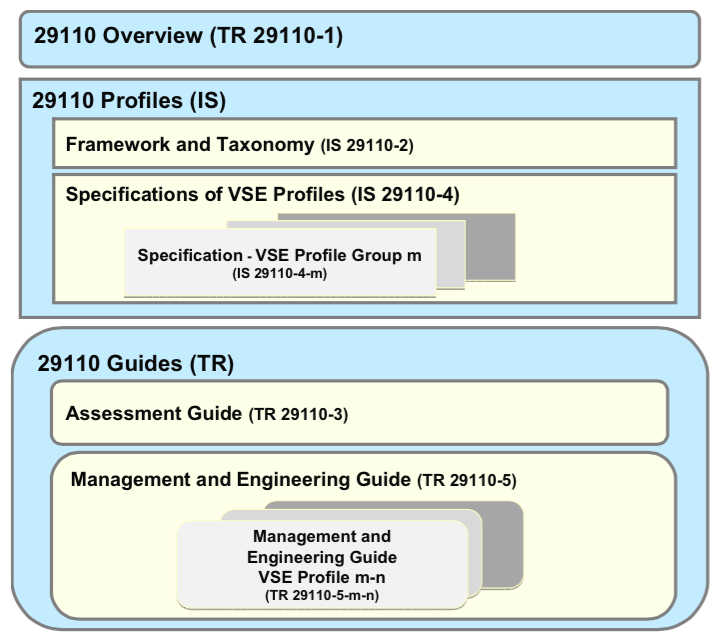
\includegraphics[scale=0.4]{figuras/serie_iso.png}
\caption{Série \iso \cite[pág. 7]{iso}}
\label{fig:serie:iso}
\end{figure}

O guia de gestão e engenharia oferece às VSE processos de \gp e \dsw que, de acordo com \cite{iso}, fazem com que os desenvolvedores ganhem benefícios através dos seguintes aspectos alcançados:

\begin{itemize}

\item Um conjunto de requisitos de projeto e produtos esperados é entregue ao cliente;

\item Um processo disciplinado de gestão que oferece visibilidade do projeto e ações corretivas para problemas e desvios de projeto é realizado;

\item Um processo sistemático e disciplinado de desenvolvimento de \sw que satisfaça as necessidades do cliente e assegure a qualidade do produto é seguido.

\end{itemize}

O guia também cita algumas condiç	ões iniciais para que a VSE possa utilizá-lo \citep{iso}:

\begin{itemize}

\item Documentação da Declaração de Trabalho do projeto;

\item Realização do estudo de viabilidade do projeto, antes do seu início;

\item Atribuição e treinamento da equipe de projeto, incluindo o gerente de projeto;

\item Disponibilidade de bens, serviços e infraestrutura para se iniciar o projeto.

\end{itemize}

Os processos de \gp e \dsw são interrelacionados, sendo a entrada do primeiro a \dt e saída do último a \swcfg, conforme pode ser observado na Figura \ref{fig:gp:dsw}. 

A \gp está ligada ao estabelecimento e controle das tarefas para se alcançar os objetivos do projeto em termos de qualidade, tempo e custo. O \dsw está relacionado às atividades de construção, integração e testes de \sw.

\begin{figure}[!h]
\centering
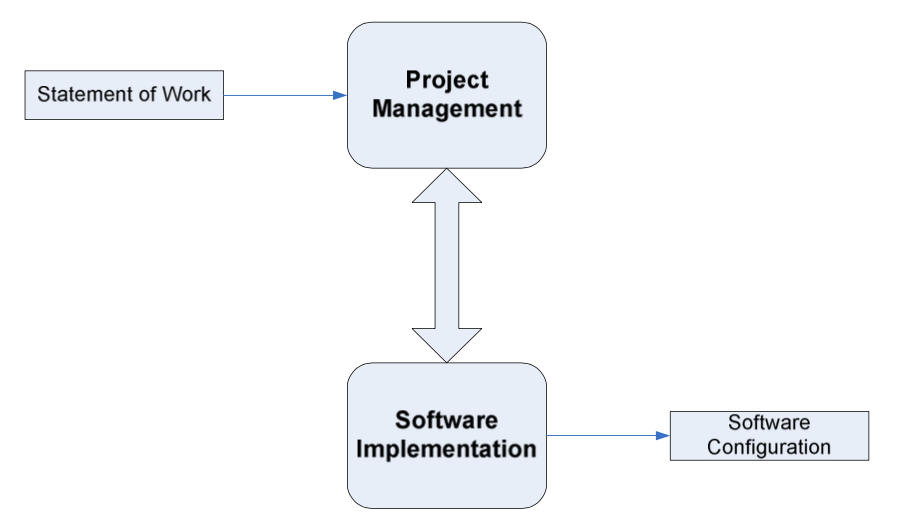
\includegraphics[scale=0.3]{figuras/gp_desenv_sw.png}
\caption{Processos básicos \cite[pág. 12]{iso}}
\label{fig:gp:dsw}
\end{figure}

\section{\gp}
\label{Sec:iso:obj:gp}

De acordo com \cite{iso}, os objetivos deste processo são:

\begin{itemize}

\item[PM.O1] O \ppj é desenvolvido de acordo com a \dt e é revisado e aceito pelo cliente. As tarefas e recursos necessários para completar o trabalho são quantificados e estimados.

\item[PM.02] O progresso do projeto é monitorado em relação ao \ppj e registrado no \prog. Correções para remediar problemas e desvios do plano são tomadas quando os objetivos do projeto não são alcançados. O fechamento do projeto é realizado para se conseguir o aceite do cliente documentado no \aceite.

\item[PM.03] A \muda é abordada através de sua recepção e análise. Mudanças aos requisitos de \sw são avaliadas em custo, cronograma e impacto técnico.

\item[PM.O4] Reuniões de revisão são realizadas com a equipe de trabalho e o cliente. Acertos são registrados e rastreados.

\item[PM.O5] Riscos são identificados conforme aparecem e durante a condução do projeto.

\item[PM.O6] Uma \vcs de \sw é desenvolvida. Itens da \swcfg são identificados, definidos e incluídos em uma \bline. Modificações e entregas de um item são controladas e disponibilizadas ao cliente e equipe de trabalho. O armazenamento, manuseio e entrega dos itens são controlados.

\item[PM.O7] A \qsw é realizada para garantir que os produtos de trabalho e processos obedeçam ao \ppj e \req.

\end{itemize}

Cada um destes objetivos pode ser alcançado através de uma série de processos que, por sua vez, irão gerar vários documentos de apoio. Os processos e o fluxo de informação que percorre estes processos podem ser resumidos na Figura \ref{fig:gp:diagr}.

\begin{figure}[!h]
\centering
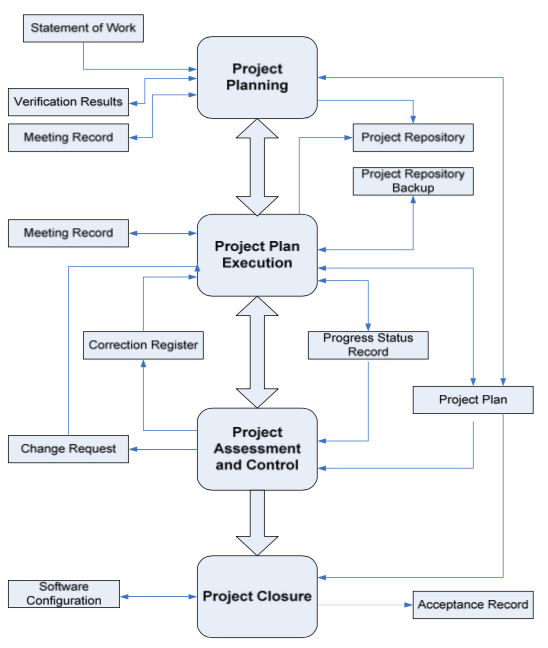
\includegraphics[scale=0.5]{figuras/gp_diagr.png}
\caption{Diagrama do processo de \gp \cite[pág. 12]{iso}}
\label{fig:gp:diagr}
\end{figure}

\section{\dsw}
\label{Sec:iso:obj:dsw}

De acordo com \cite{iso}, os objetivos deste processo são:

\begin{itemize}

\item[SI.O1] As tarefas das atividades são feitas através da realização do \ppj corrente.

\item[SI.02] Os requisitos de \sw são definidos, analisados para correção e testabilidade, aprovados pelo cliente, incluídos na \bline e comunicados.

\item[SI.03] O projeto de \sw, com arquitetura e detalhamento, é desenvolvido e incluído na \bline. Ele descreve os \comp e suas interfaces internas e externas. A consistência e rastreabilidade aos requisitos de \sw são estabelecidas.

\item[SI.O4] \comp definidos pelo projeto são produzidos. Testes unitários são definidos e realizados para verificar a consistência com os requisitos e o projeto. Rastreabilidade com os requisitos e projeto são estabelecidos.

\item[SI.O5] \Sw é produzido através da integração de \comp e verificados usando \tcase e \tproc. Resultados são registrados no \trep. Defeitos são corrigidos e a consistência e rastreabilidade com o projeto de \sw são estabelecidos.

\item[SI.O6] Uma \swcfg, que cumpra com o \req acertado com o cliente, que inclua documentações de usuário, operação e manutenção é integrada, incluída na \bline e armazenada no \rep. Necessidades de mudança na \swcfg são detectadas e os pedidos de mudança relacionados são iniciados.

\item[SI.O7] Tarefas de validação e verificação de todos os produtos de trabalho requeridos são realizadas usando os critérios definidos para se alcançar a consistência entre produtos de saída e entrada em cada atividade. Defeitos são identificados e corrigidos. Registros são armazenados nos \vvres.

\end{itemize}

Cada um destes objetivos pode ser alcançado através de uma série de processos que, por sua vez, irão gerar vários documentos de apoio. Os processos e o fluxo de informação que percorre estes processos podem ser resumidos na Figura \ref{fig:dsw:diagr}.

\begin{figure}[!h]
\centering
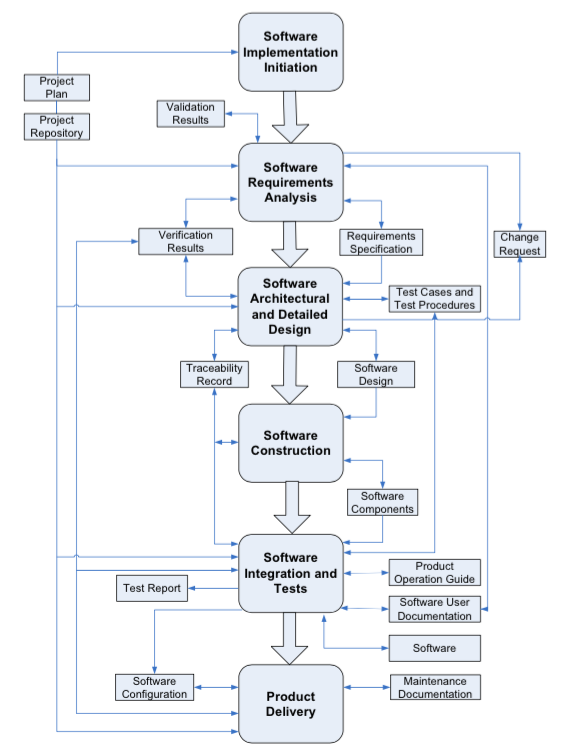
\includegraphics[scale=0.5]{figuras/dsw_diagr.png}
\caption{Diagrama do processo de \dsw \cite[pág. 30]{iso}}
\label{fig:dsw:diagr}
\end{figure}

